\section{Go garbage collector}

\begin{figure}[h!]
    \centering
    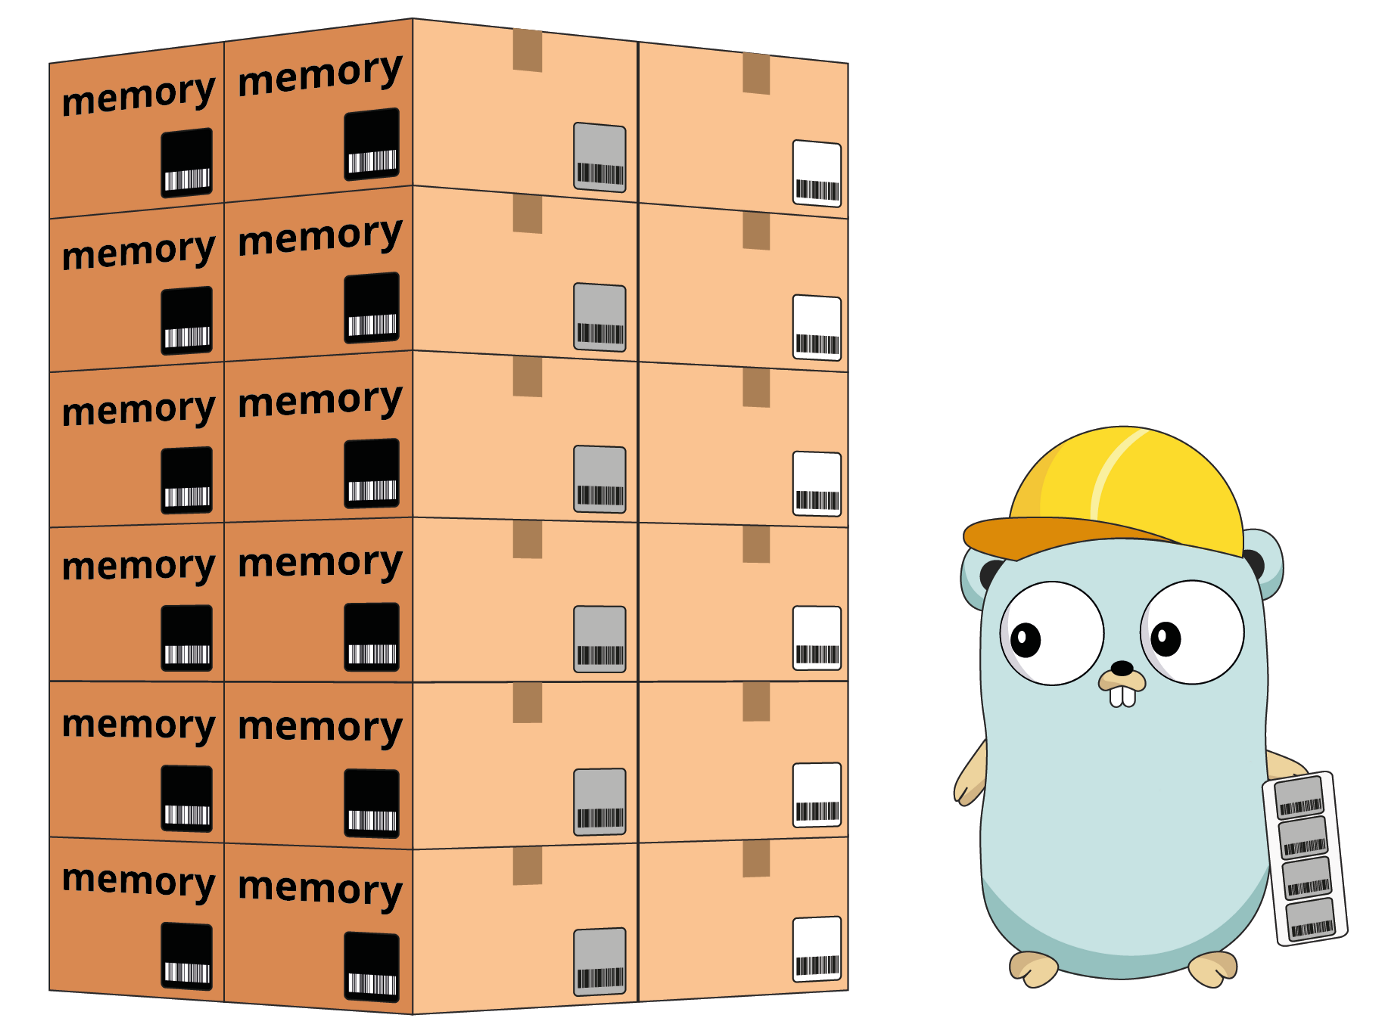
\includegraphics[width=6cm]{sections/go-garbage-collector.png}
    \caption{}
    \label{fig:my_label}
\end{figure}

Go preferisce allocare la memoria sullo stack, e quindi sullo stack di ogni goroutine, quando la variabile sullo stack non serve piu viene deallocata, questo viene garantito facendo una \textbf{escape analysis} dal compilatore prima di eseguire il codice. \newline Il garbage collector che opera sull'heap non serve in questo caso perche sappiamo la vita della variabile e quindi verra posizionata sullo stack della goroutine corrispondente.  \newline
Facciamo un esempio di un programma e cosa puo succedere:
\newpage
\begin{lstlisting}
type Oggetto struct {
    val int
}

var testOggetto = Oggetto{val: 0}

func Somma(a int, b int) int {
    return a+b
}

func Operations() {
    Var1 := 15
    Var2 := 27
    
    testOggetto.val = Somma(Var1, Var2)
}

func main() {
    Operations()
}

\end{lstlisting}

\begin{enumerate}
    \item Viene definita la variabile testOggetto e posizionata nell'heap
    \item La La funzione Operations() viene posizionata nello stack quando viene eseguita, anche le due variabili Var1 e Var2 risiedono nello stack
    \item La funzione Somma() quando viene chiamata viene posizionata nello stack
    \item Quando la funzione Somma() finisce viene tolta dallo stack
    \item Viene assegnato il valore a testOggetto.val utilizzando il puntatore della struttura che risiede nell'heap
    \item Il main esce dallo stack, rimane pero nell'heap sempre il puntatore alla testOggetto
\end{enumerate}

\begin{figure}[h!]
    \centering
    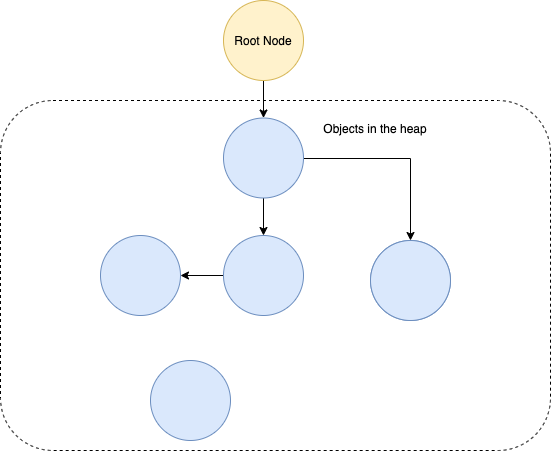
\includegraphics[width=7cm]{sections/go-garbage-heap.png}
    \caption{Heap e gli oggetti}
    \label{fig:my_label}
\end{figure}

Ora che abbiamo il puntatore nell'heap, sara' compito del garbage collector a riconoscere che non ci serve piu occupare quello spazio di memoria. \newline
Il garbage collector del Go si divide in due parti, il \textbf{mutator} e \textbf{collector}. \newline
Il collector esegue la logica del garbage collection, trova gli oggetti che dovrebbero essere liberati. \newline
Il mutator alloca nuovi oggetti nell'heap e inoltre lo aggiorna durante l'esecuzione del programma. Durante l'aggiornamento dell'heap gli oggetti potrebberro essere resi irragiungibili dall'heap perche non servono piu. Per esempio dall'immagine sopra l'oggetto in fondo viene staccato dall'heap dal mutator e sucessivamente eliminato dal collector.

\subsection{Implementazione del garbage collector}

Il garbage collector di go e': \textbf{non-generational concurrent, tri-color mark e sweep garbage collector.} \newline Cosa significa?
\begin{itemize}
    \item generational: significa che il garbage collector alloca gli oggetti sullo stak se si conosce per quanto verranno utilizzati, ma questo Go gia lo fa nel compilatore infatti non ne ha bisogno. \newline
    concurrent: significa che il collector viene eseguito in concorrenza con i thread del mutator.
    \item mark e sweep e' il tipo di garbage collector. \newline
    Nella fase mark il collector attraversa l'heap e marchia gli oggetti che non servono piu. \newline
    Nella fase di sweep vengono rimossi gli oggetti marchiati.
    \item tri-color e' il tipo di algoritmo utilizzato.
\end{itemize}

\begin{figure}[h!]
    \centering
    
\includegraphics[width=8cm]{sections/runtime-go.png}
    \caption{runtime go}
    \label{fig:my_label}
\end{figure}

Go implementa l'algoritmo nel modo seguente:

\begin{enumerate}

    \item Go fa raggiungere a tutte le goroutine un punto sicuro chiamato \textbf{stop the world}. Qua si ferma temporaneamente il programma e attiva una \textbf{white barrier} che mantiene l'integrita dell'heap. Questo permette al collector e alle goroutine di lavorare simultaneamente
    
     \begin{figure}[!h]
        \centering
        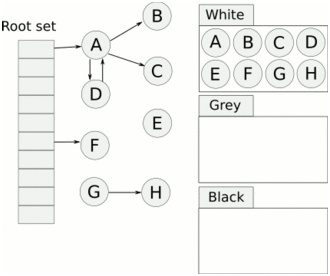
\includegraphics[width=6cm]{sections/frame0.png}
        \caption{Caption}
        \label{fig:my_label}
    \end{figure}
    
    \item Una volta che tutte le goroutine hanno la white barrier attiva, Go inizia \textbf{starts the world} e ha dei workers che lavorano per il garbage collector.
    
    \begin{figure}[!h]
        \centering
        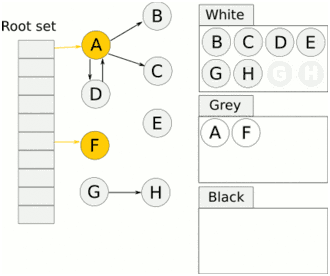
\includegraphics[width=6cm]{sections/frame1.png}
        \caption{Caption}
        \label{fig:my_label}
    \end{figure}
    
    \item La fase di marking viene eseguita implementando il \textbf{tri-color algorithm}. Quando inizia la fase tutti gli oggeti sono bianchi tranne per il nodo di root che viene marchiato di grigio. Quindi il garbage collector inizia a scannerizzare gli stacks, le variabili globali e i puntatori all'heap per vedere quali sono in uso. \newline
    Tutti gli oggetti che vengono trovati vengono marchiati di grigio e si possono far ripartire le goroutine.
    
    \begin{figure}[!h]
        \centering
        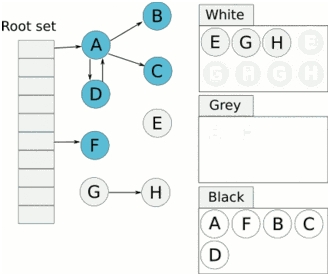
\includegraphics[width=6cm]{sections/frame2.png}
        \caption{fase 3}
        \label{fig:my_label}
    \end{figure}
    \newpage
    \item Gli oggetti marchiati di grigio vengono marchiati di nero. Gli oggetti che rimangono bianchi vengono puliti dal collector ma dopo aver fermato tutte le goroutine. \newline
    Ora il programma puo continuare con la sua normale esecuzione.
    
    \begin{figure}[!h]
        \centering
        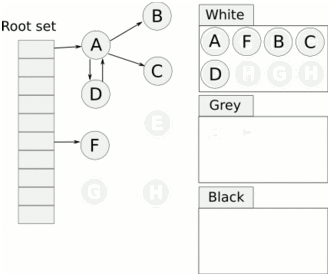
\includegraphics[width=6cm]{sections/frame3.png}
        \caption{fase 4}
        \label{fig:my_label}
    \end{figure}
    
    
\end{enumerate}






